\section{Methods}

To archive clustering, the method adopted was to compare document using the authorship linkings strategies presented in \cite{kocher_verification}.
In \cite{kocher_verification} the authors compared multiple text representation based on author style : words frequencies, lemma frequencies, Part-Of-Speach (POS) tags frequencies, short sequences of POS tags, as well as n-grams frequencies.
The distance mesures used are : $L^1$ norms (Manhattan, Tanimoto), $L^2$ norm (Matusita, Clark), inner products (Cosine distance) and the Jeffery divergence.
Depending on the dataset, the text representation and the metric used, no clear text representation and different distance mesures were giving better or worse results.

In this study to archive a good clustering, the main objective is to have a reliable authorship linking rank list.
To try to increase the quality of the rank list, the proposed method is to use a combination of multiple rank list using different strategies to form a hopefully better rank list.
By using the most diverse strategies, we belive it is possible to increase the quality using the principle of combinaison of evidences.

\subsection{Authorship linking}

The next sections will present, different stylistic text representations to create the authorship linking rank list. They are mostly based on the text representation proposed in \cite{kocher_verification}.

\subsubsection{Word Tokens}

The first method is rather simple but yet effective where we consider each token as a word.
In the datasets used the tokenization is already done such that each word is corretly tokenized.

\subsubsection{Letters n-grams}

For this method, instead of considering every token as a word, we create word from short sequences of letters called n-grams using Definition~\ref{def:n-grams}.
To consider overlapping word, the whole document is synthetized to a long string by joining every token by a \textit{underscore} : $\_$.

\begin{definition}[$N$-Grams]
  \label{def:n-grams}
  A $N$-gram is a special type of tokenization which is constructed by creating a token for the substrings from $0$ to \textit{text\_size} - $N$ of size $N$.
  Example: Using 3-grams The string: "brown fox" is converted to: \\
  $("\text{bro}", "\text{row}", "\text{own}", "\text{wn\_}", "\text{n\_f}", "\text{\_fo}", "\text{fox}")$
\end{definition}


\subsubsection{POS n-grams}

To detect another stylistic aspect of a text, this method aim to consider the sentence constructions of the authors using short sequences (n-grams) of POS tags.

For example, the sentence : \textit{"The cat eat a fish"} has the following POS tag \textit{"Article Noun Verb Article Noun"} which correspond to the following 3-gram of POS : \textit{"Article Noun Verb"} / \textit{"Noun Verb Article"} / \textit{"Verb Article Noun"}.
In practice the POS is more detailed, for example instead of just considering the verb, the verb and it's tense can be used, same for the other type of POS.

Figure~\ref{fig:pos_ngrams} show the average precision on the rank list produced by using POS n-grams over the number of MFW (most frequent word, in this case POS n-grams are considered as words).
The two following informations can be intuitively observed on this plot:

A more complex POS n-gram requirement more MFW to archive its maximal effectiveness.
In the St-Jean corpus 26 POS are used to describe every words in the corpus.
Which correspond to $26^2 = 676$ possible unique POS 2-grams, to $26^3 = 17'576$ POS 3-grams and $26^4 = 456'976$.

Like the other methods, an overfit to less important words is possible if the MFW ceiling is too high, reducing the average precision.
In Figure~\ref{fig:pos_ngrams} the POS 2-grams clearly have drop in average precision after \~250-MFW.

\begin{figure}
  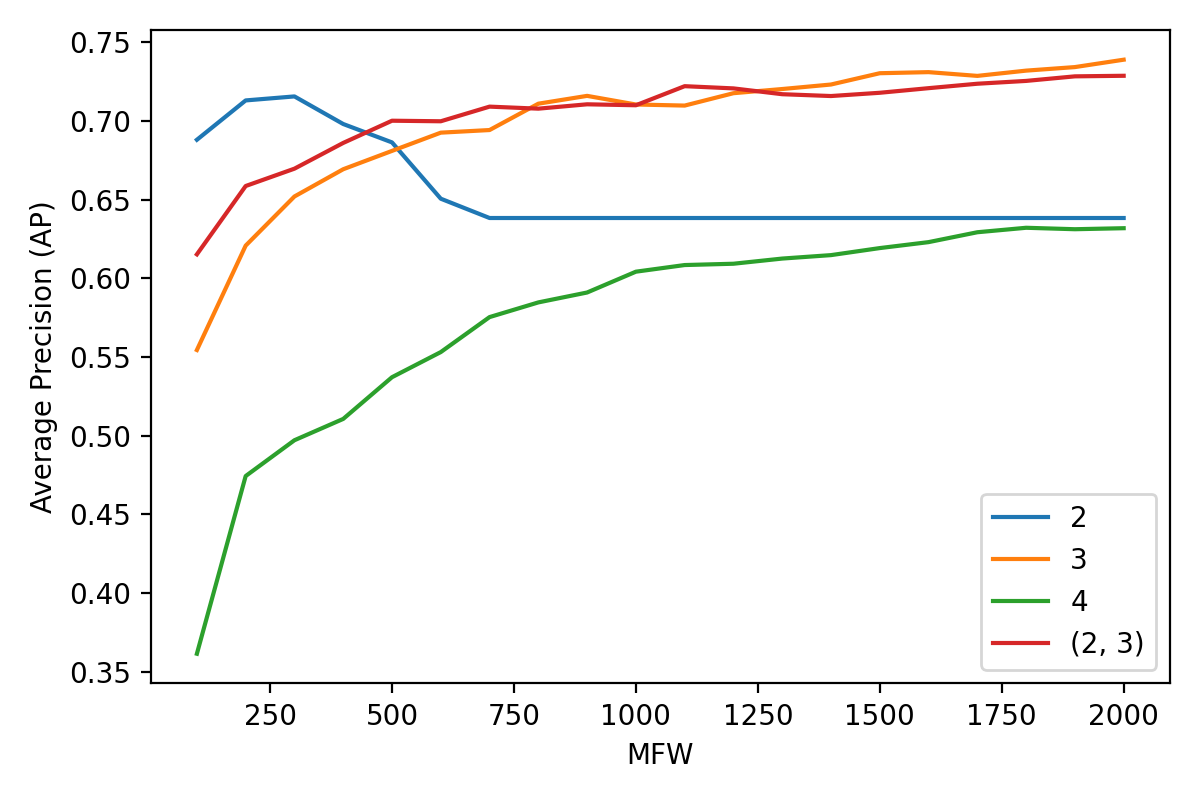
\includegraphics[width=\linewidth]{img/pos_ngrams.png}
  \caption{Average precision over the MFW in the rank list generated using the z-score normalized cosine distance.}
  \label{fig:pos_ngrams}
\end{figure}

\subsubsection{First letters, last letters of tokens}

With this methods, the goal is to extract the N first letter of each word tokens which correspond generaly to the meaning of a word.
This approach is closely related to the lemma approach.
Extract also the N last letter of each word tokens which in this case correspond to the role of the word in a sentence.
This second approach is closely related to the POS approach.

These two methods can be considered as simplified n-grams approach of the same size.

Figure~\ref{fig:first_last_letters_ngrams} shows the average precision using the z-normalized cosine distance on the experiment for N = 4.

\begin{figure}
  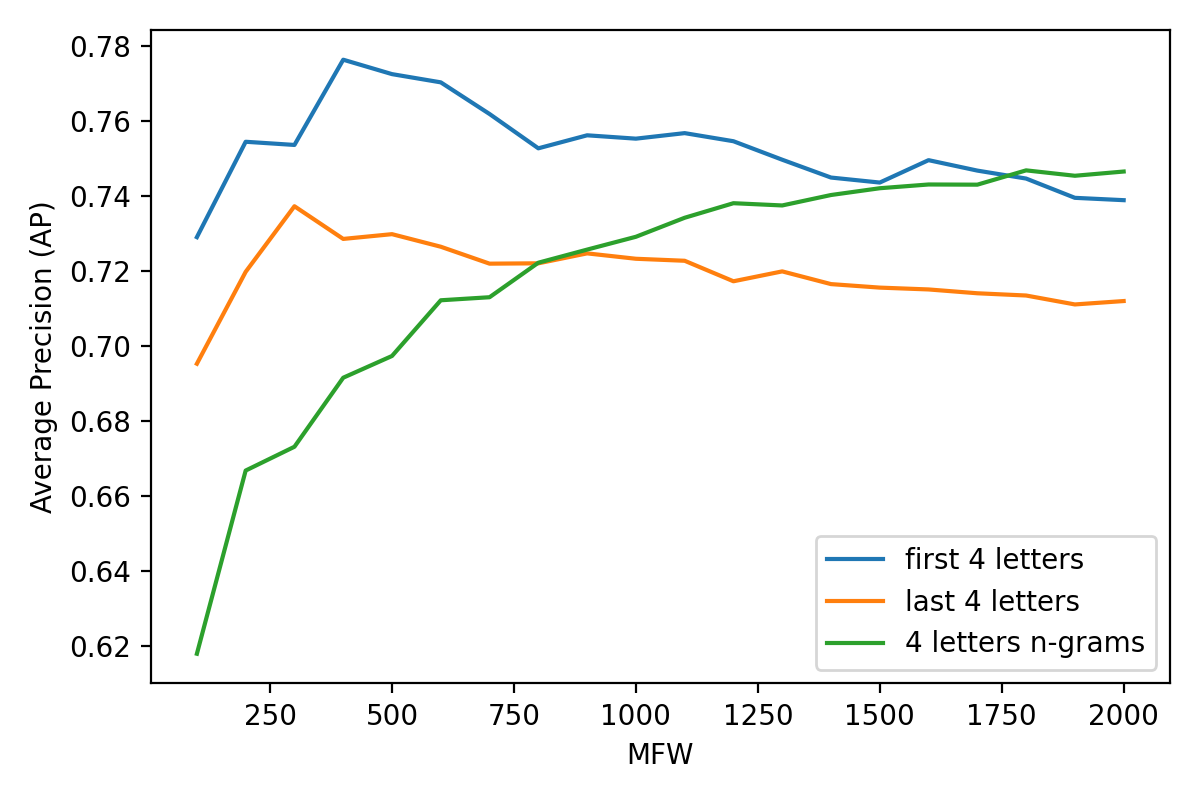
\includegraphics[width=\linewidth]{img/first_last_letters_ngrams.png}
  \caption{Average precision over the MFW in the rank list generated using the z-score normalized cosine distance.}
  \label{fig:first_last_letters_ngrams}
\end{figure}


\subsubsection{Frequent errors}

This section, try to understand the errors in our system, in this case the false links (document pairs with different authors) highly ranked on different rank list.
The system is highly based on the feature vector created using the N-MFW

Using the St-Jean dataset, to find reccurant errors in our system we use 5 different distance metrics on the relative frequency of the 500-MFW.
This generate 5 rank lists.
The average precision for these rank list is always greater than 0.7.

With this 5 rank lists only the top 15 incorrect pairs are kept to be analyzed, this correspond to the most inaccurate pairs.
The Tables~\ref{tab:errors1}~/~\ref{tab:errors2}/~\ref{tab:errors3} show the 10-MFW relative frequency in the top 15 of the rank lists.
These pairs are found using 500-MFW but for visibility purpose we only show the 10-MFW.
These tables clearly show similarities in style for these texts pairs.
Using a distance function on these two vectors will produce a low score and thus rank them high in the rank list.

Since the style is close using MFW on the token as a metric, we can't clearly determinate that these texts are from different author using only this type of representation.

\begin{table}
  \caption{Relative term frequencies of the top 10 words in Zola (49) / Flaubert (63), in the 15 incorrect of 4 out of 5 rank lists}
  \label{tab:errors1}
  \begin{tabular}{|l|c|c|}
      \hline
      Word & Zola (49) & Flaubert (63) \\
      \hline
      , & 0.328 & 0.312 \\
      . & 0.136 & 0.129 \\
      de & 0.117 & 0.103 \\
      la & 0.083 & 0.078 \\
      il & 0.082 & 0.067 \\
      le & 0.060 & 0.059 \\
      et & 0.048 & 0.070 \\
      elle & 0.042 & 0.070 \\
      à & 0.049 & 0.061 \\
      les & 0.055 & 0.051 \\
      \hline
  \end{tabular}
\end{table}

\begin{table}
  \caption{Relative term frequencies of the top 10 words in Maupassant (43) / Flaubert (52), in the 15 incorrect of 4 out of 5 rank lists}
  \label{tab:errors2}
  \begin{tabular}{|l|c|c|}
      \hline
      Word & Maupassant (43) & Flaubert (52) \\
      \hline
      , & 0.305 & 0.316 \\
      . & 0.126 & 0.134 \\
      de & 0.133 & 0.100 \\
      et & 0.081 & 0.078 \\
      la & 0.070 & 0.080 \\
      il & 0.061 & 0.066 \\
      à & 0.061 & 0.061 \\
      le & 0.056 & 0.062 \\
      elle & 0.059 & 0.055 \\
      l' & 0.048 & 0.047 \\
      \hline
  \end{tabular}
\end{table}

\begin{table}
  \caption{Relative term frequencies of the top 10 words in Maupassant (10) / Flaubert (52), in the 15 incorrect of 4 out of 5 rank lists}
  \label{tab:errors3}
  \begin{tabular}{|l|c|c|}
      \hline
      Word & Maupassant (10) & Flaubert (52) \\
      \hline
      , & 0.299 & 0.317 \\
      . & 0.136 & 0.135 \\
      de & 0.110 & 0.101 \\
      et & 0.090 & 0.078 \\
      il & 0.089 & 0.066 \\
      la & 0.069 & 0.080 \\
      le & 0.061 & 0.062 \\
      à & 0.057 & 0.061 \\
      - & 0.045 & 0.052 \\
      l' & 0.044 & 0.047 \\
      \hline
  \end{tabular}
\end{table}


\subsubsection{Rank list fusion}

Each rank list is ordered using a different distance measure.
The order of magnitude of each rank list is different.
To avoid this problem, the solution opted is to only use the rank of each link.

An additional constraint desired is to favor top ranked link and penalize bottom ranked links when fusing rank lists.
This constraint can be easily explained by observing the distance over the rank graph of the rank list.
Figure~\ref{fig:distance_over_rank} clearly show us the top ranked links and bottom ranked links are fewer than the middle section.

\begin{figure}
  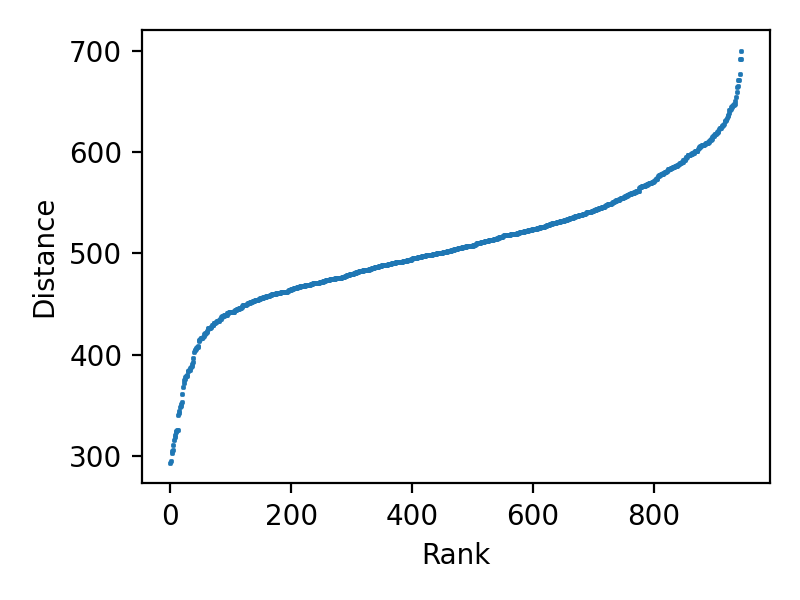
\includegraphics[width=\linewidth]{img/distance_over_rank.png}
  \caption{Distance over rank in the links of the Brunet dataset using Manhattan distances using the 500 most frequent tokens.}
  \label{fig:distance_over_rank}
\end{figure}

Which correspond to correctly correlated documents (top links) and negatively correlated documents (bottom links).
Assuming that the top rank are true links after the rank list fusion these link should also be top rank.
The same reasoning can be apply for the bottom links.

Using the reciprocal of the sigmoid function we can modelize such curve. Sigmoid functions presented in Equation~\ref{eq:sigmoid} and Figure~\ref{fig:sigmoid}. It's reciprocal in Equation~\ref{eq:sigmoid_r} and Figure~\ref{fig:sigmoid_reciprocal}

\begin{equation}
  \label{eq:sigmoid}
  S(x) = \frac{1}{1+e^-x}
\end{equation}
\begin{equation}
  \label{eq:sigmoid_r}
  S^{-1}(x) = -\ln{\frac{x-1}{x}}
\end{equation}

\begin{figure}
  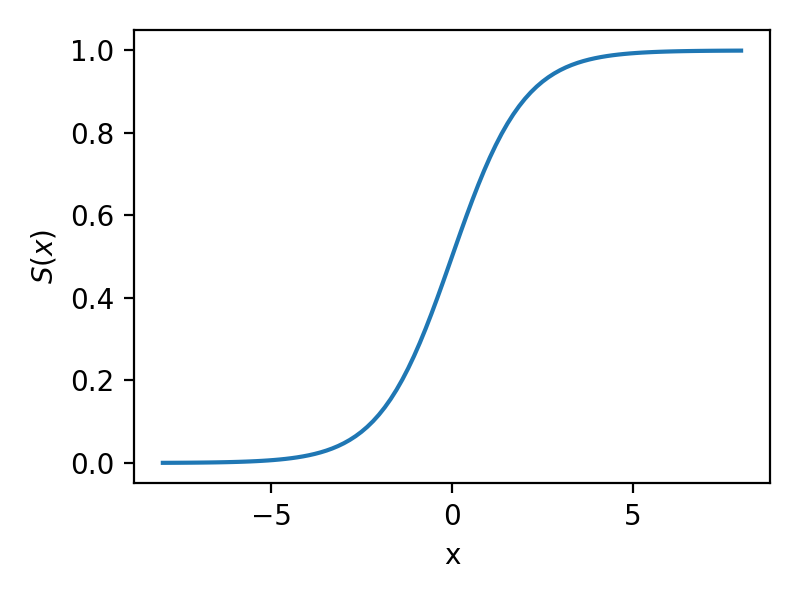
\includegraphics[width=\linewidth]{img/sigmoid.png}
  \caption{Sigmoid function between -8 and 8}
  \label{fig:sigmoid}
\end{figure}
\begin{figure}
  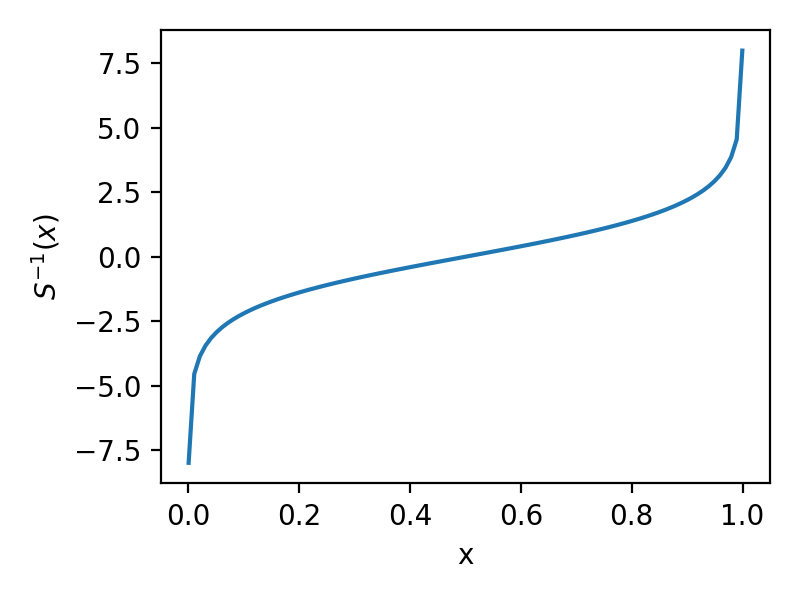
\includegraphics[width=\linewidth]{img/sigmoid_reciprocal.png}
  \caption{Reciprocal of the sigmoid function between sigmoid(-8) and sigmoid(8)}
  \label{fig:sigmoid_reciprocal}
\end{figure}

\subsection{Authors Clustering}

To find clusters of authors, a possible way is to use aglomeratives clustering on a rank list.
